\newpage

\chapter{My Notebook}

\section{Start importing}

\begin{lstlisting}[language=JuliaLocal, style=julia]
using Plots
using Makie
using CairoMakie
using Distributions
using DataFrames
\end{lstlisting}

\subsection{Some theory}
The Wasserstein Distance for 1D distributions can be obtained by:  $$ \int_0^1 |C_\alpha^{-1}(r) - C_\beta^{-1}(r)|^p dr  $$  Where  $C_\alpha^{-1}$ is the quantile function for the distribution  $\alpha$ (the inverse of the Cumulative Distribution Function).
\begin{lstlisting}[language=JuliaLocal, style=julia]
μ(x) = pdf(Normal(0,2),x)
println("Myplot")
Plots.plot(μ)
\end{lstlisting}

\begin{verbatim}
Any["Myplot\n"]
\end{verbatim}

% \begin{figure}[H]
% 	\centering
% 	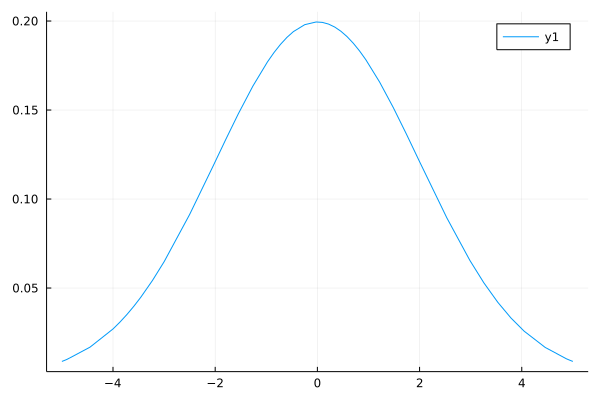
\includegraphics[width=0.8\textwidth]{./figures/jupyternotebook_figure1.svg}
% 	\label{fig:jupyternotebook_figure1.svg}

% \end{figure}

\begin{lstlisting}[language=JuliaLocal, style=julia]
Makie.lines(-10:0.1:10, μ.(-10:0.1:10))
\end{lstlisting}

\begin{figure}[H]
	\centering
	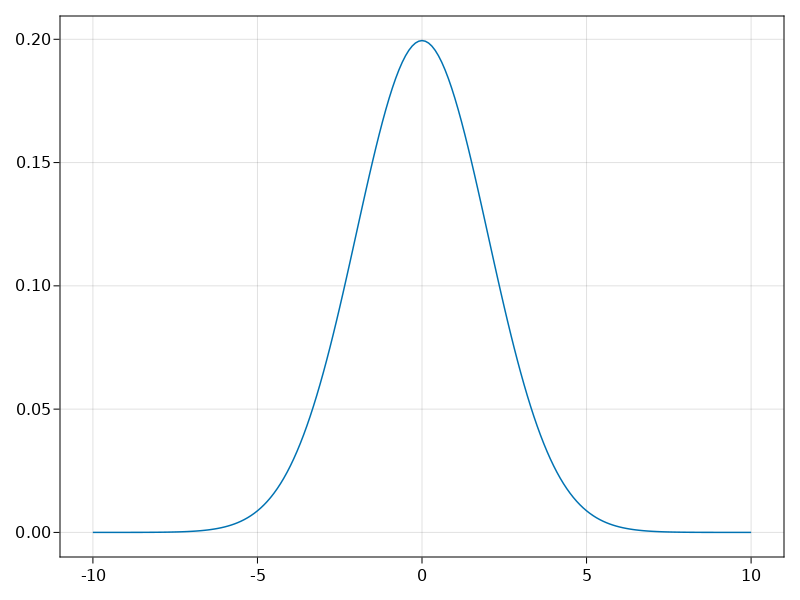
\includegraphics[width=0.8\textwidth]{./figures/jupyternotebook_figure2.png}
	\label{fig:jupyternotebook_figure2.png}

\end{figure}

\begin{lstlisting}[language=JuliaLocal, style=julia]
function example(μ)
    for i in 1:10
        println(μ(i))
    end
end
example(μ)
\end{lstlisting}

\begin{verbatim}
Any["0.17603266338214976\n", "0.12098536225957168\n", "0.06475879783294587\n", "0.02699548325659403\n", "0.00876415024678427\n", "0.0022159242059690038\n", "0.0004363413475228801\n", "6.691511288244268e-5\n", "7.991870553452737e-6\n", "7.433597573671488e-7\n"]
\end{verbatim}

\begin{verbatim}
Any["0.17603266338214976\n", "0.12098536225957168\n", "0.06475879783294587\n", "0.02699548325659403\n", "0.00876415024678427\n", "0.0022159242059690038\n", "0.0004363413475228801\n", "6.691511288244268e-5\n", "7.991870553452737e-6\n", "7.433597573671488e-7\n"]
\end{verbatim}

\begin{lstlisting}[language=JuliaLocal, style=julia]
rand(10)
\end{lstlisting}

\begin{lstlisting}[language=JuliaLocal, style=julia]
μ;
\end{lstlisting}
\href{figure.svg}{Figure}  \href{plotexample.png}{Figure2}
\begin{lstlisting}[language=JuliaLocal, style=julia]
DataFrame(x=rand(10),y=rand(10))
\end{lstlisting}

\begin{tabular}{r|cc}
	   & x         & y         \\
	\hline
	   & Float64   & Float64   \\
	\hline
	1  & 0.0326174 & 0.589007  \\
	2  & 0.368715  & 0.690396  \\
	3  & 0.366451  & 0.803439  \\
	4  & 0.212434  & 0.581906  \\
	5  & 0.140433  & 0.678201  \\
	6  & 0.329857  & 0.50792   \\
	7  & 0.828484  & 0.0507595 \\
	8  & 0.480084  & 0.021381  \\
	9  & 0.784926  & 0.504361  \\
	10 & 0.43102   & 0.316321  \\
\end{tabular}

\begin{lstlisting}[language=JuliaLocal, style=julia]

\end{lstlisting}
